%!TEX root = pset2.tex

\section{Titanic Data}\label{sec:tinanic}

\subsection{Logistic Regression}
We use Logistic Regression classifier on the Titanic data to make predictions on survivor results. Before running the regression, we scale the features in two ways: 1) standardizing using mean and standard deviation by $(X_{j}^{(i)} - \mu(X_{j}))/\sigma(X_{j})$; 2) scale so each dimension is within the $[0, 1]$ range using min and max: $(X_{j}^{(i)} - \min{X_j})/(\max{X_j} - \min{X_j})$. We find the scaling constants in the training sets only, and use the same constants in the validation and testing sets. Note comparing the two scaling methods is simply for exploration purposes and we are not choosing one or the other in the model selection process.

With no regularization, we obtain a testing set accuracy of $77.78\%$ in both cases of scaling methods. To find the best $\lambda$, we use the cross validation technique. The validation set accuracy with respect to $\lambda$ is presented in Figure \ref{fig:3_LR_cv}. We therefore choose $\lambda = 10$ in standard-deviation-based scaling, and $\lambda = 0.1$ in range-based scaling. on the validation accuracy. The test set accuracy is then $75.13\%$ and $76.19\%$, respectively. Unfortunately neither is not as good as the non-regularized logistic regression. Furthermore, the way how one scales the features can also impact the accuracy.

\begin{figure}[hb]
\centering
	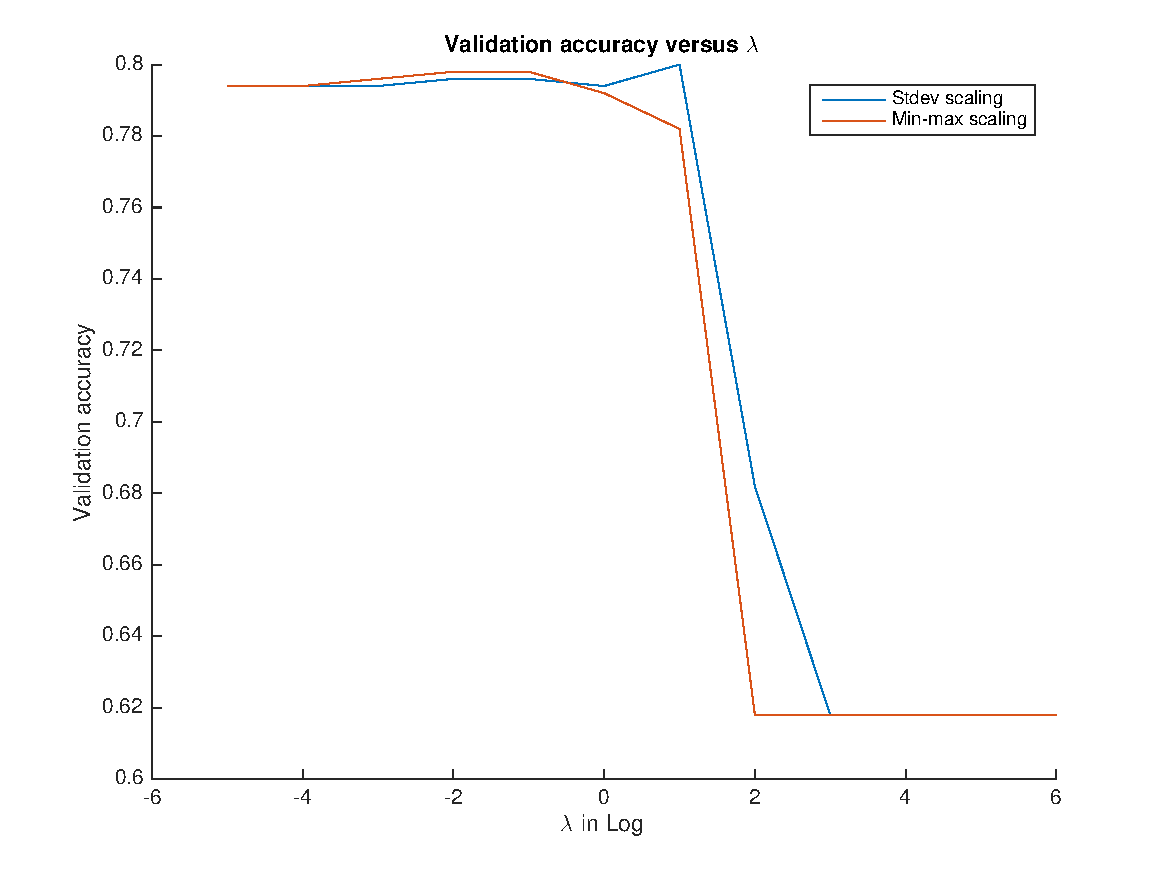
\includegraphics[scale=0.4]{hw2_3_cv.pdf}
	\caption{Tinanic Data, Cross validation error in logistic regression with respect to $\lambda$, under two different scaling methods.}\label{fig:3_LR_cv}
\end{figure}


\subsection{SVM}
TODO

\subsection{Comparison}
TODO compare LR and SVM

The estimated coefficients for logistic regression and SVM are presented in Table \ref{tab:titanic_coeff}. Since we do not have standard error and confidence interval information, we can only rely on the magnitude of the estimator (even if they are not statistically significant). 

We observe that being woman, higher class and higher fare are associated with higher likelihood of survival, whereas being 3rd class is strongly associated with death. 

\begin{table}[h!]
\centering
\caption{Estimated logistic regression coefficients in Titanic data, $\lambda = 10$}
\begin{tabular}{llr}
	\hline 
	Coefficient & Description & Logistic estimator \\
  \hline
  $w_0$  & Constant &-0.6289 \\
  $w_1$ 	& Passenger class 1 & 0.1680\\
  $w_2$ 	& Passenger class 2	  & 0.2013\\
  $w_3$  & Passenger class 3 & -0.3245\\
  $w_4$ 	 & Sex & 0.7795\\
  $w_5$ 	 & Age & -0.1417\\
  $w_6$ 	 & Num siblings/Spouses aboard & -0.0477 \\
  $w_7$ 	 & Num parents/children aboard & 0.1422\\
  $w_8$ 	 & Pasenger fare & 0.1533\\
  $w_9$ 	 & Port of embarkation = Southampton & -0.0955\\
  $w_{10}$  & Port of embarkation = Cherbourg & 0.1090\\
  $w_{11}$ & Port of embarkation = Queenstown	& 0.0393	\\
  \hline
\end{tabular}\label{tab:titanic_coeff}
\end{table}




